\section{Results}

\subsection{The isolation rate tracks the true coverage}

In the synthetic Zipf mixtures every document belongs to a known topic, so we know exactly which percentage of the topics a sample has covered. Over four settings of the mixture, three random seeds and eleven sample sizes from 50 to 5{,}000, the coverage $1 - G$ at a resolution of half the median distance between documents in a pilot follows the true topic coverage closely. The rank correlation is $\rho = 0.968$, and $1 - G$ is off by 2.9 percentage points on average. At smaller resolutions the agreement falls away, because two documents of the same topic often lie farther apart than $r$. The resolution must therefore match the question being asked of the sample.

\subsection{The isolation rate collapses on $n r^{d/2}$}
\label{sec:collapse}

Table~\ref{tab:collapse} reports the fit of Equation~\ref{eq:collapse} on 17 pairs of corpus and encoder, and Figure~\ref{fig:collapse} shows six of them. On ten pairs the law holds: the three synthetic manifolds, AskDocs and TIFU under both encoders, the random slice of the Census tweets, Truth Social and Bluesky. On these ten, a fit on samples of up to 1{,}000 documents explains 92\% or more of the variance of $\log(-\log G)$ in samples of up to 7{,}000 documents. In terms of $G$ itself, the law predicts the isolation rate of the largest sample with an average error between 1.5 and 4.2 percentage points on these ten pairs. A researcher who has drawn a few hundred documents can thus predict from them alone what percentage of a sample twenty times larger will be isolated, at every resolution at once.

For AskDocs and TIFU, the points of all colours in Figure~\ref{fig:collapse} lie on one curve once the horizontal axis is $n r^{d/2}$, so that a larger sample and a looser resolution are interchangeable. For Trump and for the Zipf mixture, each colour traces its own curve, and no single $d$ brings them together. The second estimate of $d$, from the separate coefficients on $\log n$ and $\log r$, differs from the TwoNN estimate by at most 19\% on the ten passing pairs, and by 27\% to 46\% on the seven failing pairs.

The law also predicts better than the two obvious alternatives, both fitted on the same samples of up to 1{,}000 documents. A separate curve in $n$ at each resolution, which needs no $d$, has 1.5 to 3.8 times the average error of the law on nine of the ten passing pairs. The law wins because it pools the information from all resolutions through one $d$. The extrapolation of \citet{chao2012coverage}, the standard ecological tool, run within its recommended range, has 2 to 9 times the average error of the law on the passing pairs.

\begin{figure*}[t]
\centering
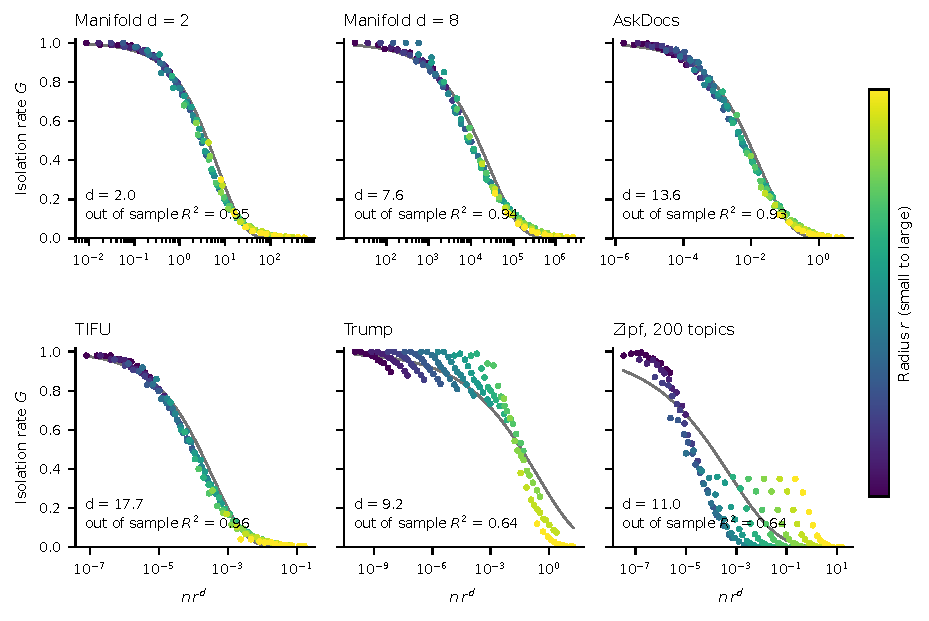
\includegraphics[width=\textwidth]{figures/collapse.pdf}
\caption{Isolation rate $G$ against $n r^{d/2}$ (log scale; $n r^{d}$ on the manifolds, which use Euclidean distance), one panel per corpus, with the GTR encoder for the three forum corpora. Each point is one sample size at one resolution, and the colour gives the resolution, from the 5th (dark) to the 99th (light) percentile of the nearest neighbor distances in a pilot. Where the law holds (the synthetic manifolds, AskDocs, TIFU), points from all resolutions fall on one curve. Where it fails (Trump, the Zipf mixture), the points of each resolution form their own curve. The grey line is the fit of Equation~\ref{eq:collapse} on samples of up to 1{,}000 documents. Each panel gives $d$ and the full out of sample $R^2$ from Table~\ref{tab:collapse}.}
\label{fig:collapse}
\end{figure*}

\begin{table*}[t]
\centering
\small
\setlength{\tabcolsep}{5pt}
\begin{tabular}{llrrrrrrrr}
\toprule
Corpus & Encoder & $N$ & $d$ (sd) & $d$, ratio & $b$ & $R^2$ pilot & $R^2$ full & error, law & error, per resolution \\
\midrule
AskDocs & Qwen3 & 10{,}000 & 25.5 (0.78) & 24.4 & 0.54 & 0.98 & 0.99 & 0.015 & 0.057 \\
Truth Social & Qwen3 & 50{,}000 & 25.3 (0.30) & 28.9 & 0.43 & 0.98 & 0.98 & 0.025 & 0.053 \\
Census random & Qwen3 & 7{,}610 & 25.7 (0.78) & 24.8 & 0.27 & 0.98 & 0.97 & 0.040 & 0.025 \\
Manifold $d{=}2$ & none & 20{,}000 & 2.0 (0.05) & 2.4 & 0.80 & 0.97 & 0.96 & 0.027 & 0.065 \\
TIFU & Qwen3 & 10{,}000 & 27.3 (0.70) & 26.8 & 0.53 & 0.98 & 0.96 & 0.039 & 0.086 \\
Bluesky & Qwen3 & 50{,}000 & 32.0 (1.38) & 30.4 & 0.42 & 0.98 & 0.96 & 0.037 & 0.056 \\
TIFU & GTR & 10{,}000 & 36.5 (0.66) & 38.1 & 0.50 & 0.97 & 0.95 & 0.040 & 0.070 \\
Manifold $d{=}8$ & none & 20{,}000 & 8.0 (0.21) & 8.1 & 0.62 & 0.97 & 0.95 & 0.042 & 0.081 \\
AskDocs & GTR & 10{,}000 & 27.3 (0.71) & 27.1 & 0.51 & 0.98 & 0.95 & 0.042 & 0.087 \\
Manifold $d{=}4$ & none & 20{,}000 & 4.0 (0.16) & 4.3 & 0.72 & 0.96 & 0.92 & 0.036 & 0.091 \\
\midrule
Census illegal & Qwen3 & 17{,}202 & 22.8 (0.66) & 15.0 & 0.26 & 0.93 & 0.85 & 0.026 & 0.053 \\
Census covid & Qwen3 & 17{,}837 & 21.3 (0.80) & 14.4 & 0.30 & 0.85 & 0.79 & 0.045 & 0.073 \\
Trump & Qwen3 & 10{,}000 & 17.9 (1.02) & 10.5 & 0.26 & 0.90 & 0.78 & 0.045 & 0.075 \\
Census trump & Qwen3 & 30{,}136 & 18.0 (1.68) & 12.6 & 0.26 & 0.87 & 0.78 & 0.043 & 0.056 \\
Census citizens & Qwen3 & 7{,}849 & 18.1 (0.48) & 13.2 & 0.27 & 0.76 & 0.73 & 0.043 & 0.058 \\
Trump & GTR & 10{,}000 & 17.9 (0.97) & 10.4 & 0.27 & 0.79 & 0.63 & 0.054 & 0.069 \\
Zipf, 200 topics & none & 20{,}000 & 22.7 (0.70) & 12.9 & 0.21 & 0.66 & 0.62 & 0.136 & 0.026 \\
\bottomrule
\end{tabular}
\caption{The collapse law on 17 pairs of corpus and encoder, sorted by the full out of sample $R^2$. Pairs above the line pass the pilot test. $d$: intrinsic dimension by TwoNN with Euclidean distance between unit embeddings (Euclidean distance on the manifolds), mean and standard deviation over five pilots of 2{,}000 documents (over three samples of the source for the GTR forum corpora). $d$, ratio: the second estimate of $d$, from the ratio of the coefficients on $\log r$ and $\log n$. $b$: shape exponent of Equation~\ref{eq:collapse}, fitted on samples of up to 1{,}000 documents. $R^2$ pilot: proportion of variance explained on subsamples of 1{,}000 to 2{,}000 documents of one pilot, by a fit on subsamples of up to 750. $R^2$ full: proportion of variance explained on samples of up to 7{,}000 documents, by a fit on samples of up to 1{,}000. Error, law and error, per resolution: average error in predicting $G$ at the largest sample, for the collapse law and for a separate curve in $n$ at each resolution.}
\label{tab:collapse}
\end{table*}

\begin{table*}[t]
\centering
\small
\setlength{\tabcolsep}{4pt}
\resizebox{\textwidth}{!}{%
\begin{tabular}{llcrrrcrrr}
\toprule
 & & \multicolumn{4}{c}{Qwen3.8-27B} & \multicolumn{4}{c}{Gemma-4-31B} \\
\cmidrule(lr){3-6}\cmidrule(lr){7-10}
Corpus & Diag. & $r_{\mathrm{same}}$ [90\%] & $n$ (\%) & pred. & interval & $r_{\mathrm{same}}$ [90\%] & $n$ (\%) & pred. & interval \\
\midrule
TIFU & pass & $\le$.05 [.05, .10] & 4{,}997 (50\%) & 50\% & 50\% & .08 [.05, .10] & 4{,}997 (50\%) & 50\% & 50\% \\
AskDocs & pass & .15 [.13, .16] & 4{,}953 (50\%) & 50\% & 50\% & .17 [.16, .19] & 4{,}923 (49\%) & 50\% & 49\% \\
Truth Social & pass & .16 [.15, .18] & 21{,}942 (44\%) & 48\% & 42\% to 45\% & .18 [.17, .20] & 20{,}610 (41\%) & 45\% & 39\% to 43\% \\
Cens.\ random & pass & .12 [.10, .18] & 3{,}352 (44\%) & 48\% & 35\% to 45\% & .28 [.26, .29] & 532 (7.0\%) & 9.2\% & 3.9\% to 11\% \\
Cens.\ covid & fail & .20 [.19, .21] & 3{,}356 (19\%) & 20\% & 17\% to 22\% & .29 [.22, .30] & 279 (1.6\%) & 1.7\% & 0.6\% to 14\% \\
Cens.\ citizens & fail & .23 [.20, .26] & 370 (4.7\%) & 4.9\% & $<$1.3\% to 10\% & .35 [.32, .38] & $<$100 ($<$1.3\%) & 0.1\% & $<$1.3\% \\
Trump (forum) & fail & .24 [.22, .26] & 442 (4.4\%) & 4.1\% & 2.2\% to 10\% & .31 [.31, .33] & $<$100 ($<$1.0\%) & 0.4\% & $<$1.0\% \\
Cens.\ trump & fail & .24 [.17, .25] & 604 (2.0\%) & 1.6\% & 1.0\% to 18\% & .31 [.29, .33] & $<$100 ($<$0.3\%) & 0.2\% & $<$0.3\% \\
Cens.\ illegal & fail & .28 [.25, .29] & $<$100 ($<$0.6\%) & 0.3\% & $<$0.6\% & .30 [.29, .32] & $<$100 ($<$0.6\%) & 0.1\% & $<$0.6\% \\
\bottomrule
\end{tabular}}
\caption{The distance that means the same content, and the random sample after which half of the corpus has a document with the same content in the sample. $r_{\mathrm{same}}$: distance at which half of the judged pairs are about the same specific content, with a 90\% interval from resampling the pairs. $n$ (\%): the sample size, measured on the whole corpus, as a count and as a percentage of the corpus. The percentage can never exceed 50\%, because the sampled half of a corpus is covered by itself. pred.: the percentage predicted from a pilot of 2{,}000 documents alone. interval: the measured percentage at the two ends of the 90\% interval of $r_{\mathrm{same}}$. $<$100: reached before the smallest sample of 100. $\le$: the crossing lies at the first bin, and 32\% of resamples find no crossing. Bluesky passes the pilot test but has no crossing, although 26\% (Qwen3.8) and 34\% (Gemma) of resamples find one. Truth Social and Bluesky are samples of 50{,}000 posts, and their percentages describe corpora of that size. Diag.: the pilot test of Section~\ref{sec:diag}.}
\label{tab:rcal}
\end{table*}

\subsection{The sample size formula}
\label{sec:nstar}

To test the formula, we treated each pair of corpus and encoder as a researcher would. We fitted Equation~\ref{eq:collapse} on samples of up to 1{,}000 documents, and Equation~\ref{eq:nstar} gave the sample size $n^{*}$ needed to bring the isolation rate down to 30\%, 20\% or 10\% at each resolution. We kept every case in which the true sample size lies beyond 1{,}000 documents, so that each case is a genuine prediction, and compared $n^{*}$ with the sample size at which $G$ actually reached the target in repeated draws. The ten passing pairs give 83 such cases.

On the ten passing pairs, the formula comes close in 77 of 83 cases, in the following sense: the sample that actually reached the target held between two thirds of $n^{*}$ and one and a half times $n^{*}$. A formula answer of 1{,}500 documents thus meant an actual need between 1{,}000 and 2{,}250 documents. When $a$ and $b$ are fitted inside one pilot of 2{,}000 documents, as a user would fit them, the formula comes close in 76 of 83 cases. On the seven failing pairs it comes close in only 10 of 23 cases. Refitting on 50 pilots gives intervals for $n^{*}$ with a median width of 19\% of $n^{*}$, which contain the true sample size in only 21\% of the cases, so the error of $n^{*}$ comes mostly from the shape of the law. We therefore report $n^{*}$ with the band observed in the tests, two thirds to one and a half times $n^{*}$, which contains the true sample size in 93\% of the cases on passing corpora.

\subsection{The pilot test}
\label{sec:diag}

The ten passing pairs reach a pilot $R^2$ of 0.96 or more, and the seven failing pairs reach at most 0.93 (Table~\ref{tab:collapse}). A threshold of 0.95 on the pilot therefore sorts every pair the same way as the full test on the whole corpus. We chose the threshold on these corpora, so it should be confirmed on others. The law should fail when the effective dimension of a corpus changes with the resolution. On Trump, clusters with a dimension near 2 hold slogans, short posts repeated in many small variations, and clusters with a dimension near 16 hold discussion. At small resolutions the isolated documents come mainly from one kind of cluster, and at large resolutions mainly from the other, so no single $d$ lines up the curves.

\subsection{The finite population correction}
\label{sec:fpc}

We compared $G$ and $G\,(1 - n/N)$ with the true missing mass $M$ on the eight forum and Census corpora under Qwen3, at sampling fractions from 1\% to 70\% of the corpus and three resolutions, 144 cases in all. Without the correction, $G$ is off by 11 percentage points on average and by as much as 49 points. With it, the estimate is off by 1.2 points on average and by at most 11 points. On random samples of 15 documents at the calibrated distances of Section~\ref{sec:rcal}, $G\,(1-n/N)$ lies within 6 percentage points of the true missing mass on every corpus, and its error averages 1.6 percentage points.

\subsection{Calibrated resolutions}
\label{sec:rcal}

On every corpus, the percentage of pairs that the judge calls the same content falls steadily as the distance grows. Where it crosses one half, however, depends on the corpus (Table~\ref{tab:rcal}). Under Qwen3.8, $r_{\mathrm{same}}$ lies at 0.05 or below on TIFU and reaches 0.28 on the Census tweets that contain the word ``illegal''. Long personal stories differ in their details even when their embeddings are close, while short posts that repeat a slogan remain the same content at a larger distance. The two judges give the same label to 71\% of pairs (Cohen's $\kappa = 0.55$), and Gemma's crossing lies farther out on every corpus. The judge is therefore part of the definition of $r$, and a user should report it together with the encoder.



Table~\ref{tab:rcal} also gives the random sample after which half of each corpus has a document with the same content in the sample. In a corpus in which no two documents share content, the sample covers only itself, so reaching this target takes exactly half of the corpus. On the Trump forum and the Census slices with the keywords citizens, trump and illegal, which repeat a few claims, at most 604 documents reach the target under either judge. On AskDocs, TIFU and Truth Social the sample must hold between 41\% and 50\% of the corpus. For these corpora, a sample covers what it contains and little more. The collapse law fitted on one pilot of 2{,}000 documents puts every corpus in the same group as the measurement.

\subsection{Choosing the documents to read}
\label{sec:design-results}

Choosing documents with the whole corpus embedded covers far more than random sampling wherever the corpus repeats itself. A random sample of 15 tweets from the Census illegal slice misses 62\% of the slice at the content level, and the same number of tweets chosen by $k$-means misses 33\%. On the Trump forum, $k$-means lowers the missing mass of a sample of this size from 88\% to 64\%. Where documents rarely have the same content as any other document, no choice of documents helps. On AskDocs at the content level, a random sample of 15 questions and a $k$-means sample of the same size both miss 99.8\% of the forum. The isolation rate $G$ of a random pilot of 100 documents predicts how much of the missing mass $k$-means removes (Spearman rank correlation $-0.90$ over 17 combinations of corpus and level). The supplementary material reports the full comparison.
